% = = = = = = = = = = = = = = = = = = = = = = = = = = = = = = = = = = = = = = = = = = = = =
% P  R  E  A  M  B  L  E
% = = = = = = = = = = = = = = = = = = = = = = = = = = = = = = = = = = = = = = = = = = = = =
\documentclass[11pt]{article}
\usepackage{amsbsy, amsmath, amssymb, authblk}

%\usepackage{array} 
%\usepackage{algorithm2e}
\usepackage{algorithmic}

\usepackage{booktabs, bm}
\usepackage[small,labelfont=bf,up,singlelinecheck=false]{caption}
\usepackage{cancel}
\usepackage{comment}
%\usepackage{fancyhdr}
%\usepackage[default]{lato}
\usepackage[T1]{fontenc}
\usepackage[bottom]{footmisc}
\usepackage{geometry}
\usepackage{graphicx}
\usepackage{hyperref}
%\usepackage[utf8]{inputenc}
%	\inputencoding{latin1}
%	\inputencoding{utf8}
%\usepackage{lettrine}
%\usepackage[sc]{mathpazo}
\usepackage{lmodern} % Nice fonts?
%\usepackage{mathrsfs}
\usepackage{mathtools} 
%\usepackage{marvosym} % silly bullet-point symbols (misc symbols)
%\usepackage{microtype}
\usepackage{minitoc}         % left in case it is needed elsewhere
\setcounter{secttocdepth}{5} % idem
\usepackage{etoc} % for toc before each section.
%\usepackage{multicol}
\usepackage{needspace}
\usepackage{paralist}
\usepackage{pifont}
%\usepackage{polynom} 			% typesetting polynomial long division
%\usepackage{setspace}
%	\onehalfspacing 
\usepackage{tocloft}
\usepackage{xparse} % DeclareDocumentCommand
\usepackage[compact]{titlesec} 		% compact shrinks whitespace around section headings.
\usepackage{ulem} 				% for strikeout \sout command.
%\usepackage{verbatim}

% Muh packagez :)
\usepackage{../Packages/MathCommands}
\usepackage{../Packages/BrandonColors}
\usepackage{../Packages/BrandonBoxes}
\usepackage{../Packages/NoteTaker}
\usepackage{../Packages/CS221}

%\usepackage{program}
% DL BOOK CONVENTIONS
\renewcommand\vec[2][]{\bm{#2}_{#1}}

\DeclareDocumentCommand{\slice}
	{ O{t} O{1} m }
	{\vec[\langle #2 \ldots #1 \rangle]{#3}}

\newcommand\myfig[2][0.3\textwidth]{\begin{figure}[h!]\centering\includegraphics[width=#1]{#2}\end{figure}}
\newcommand\myspace[1][]{\vspace{#1\bigskipamount}\Needspace{10\baselineskip}}
\newcommand\p{\Needspace{10\baselineskip} \noindent}
\newcommand\tlab[1]{\tag{#1}\label{#1}}
\newcommand\Var[1]{\mathrm{Var}\left[#1\right]}

\usepackage{layout} % Type \layout() anywhere to see values of layout frame.
%\usepackage{showframe} % Displays layout frame on all pages
\usepackage{marginnote}
\renewcommand*{\marginfont}{\scriptsize}

\usepackage{listings}

\definecolor{dkgreen}{rgb}{0,0.6,0}
\definecolor{gray}{rgb}{0.5,0.5,0.5}
\definecolor{mauve}{rgb}{0.58,0,0.82}

\lstset{frame=tb,
	language=Java,
	aboveskip=3mm,
	belowskip=3mm,
	showstringspaces=false,
	columns=flexible,
	basicstyle={\small\ttfamily},
	numbers=none,
	numberstyle=\tiny\color{gray},
	keywordstyle=\color{blue},
	commentstyle=\color{dkgreen},
	stringstyle=\color{mauve},
	breaklines=true,
	breakatwhitespace=true,
	tabsize=3
}

\usepackage{tikz}
\usetikzlibrary{arrows, automata, shapes, snakes, positioning}
\usetikzlibrary{bayesnet}


\titleformat*{\subsubsection}{\small\scshape}
\newcommand\subsub[1]{\Needspace{15\baselineskip}\hrule\subsubsection{#1}\hrule}

% O{T} means "optional with default value of `T`"
% m means mandatory argument
\DeclareDocumentCommand{\vecseq}
	{ O{T} m }
	{ \{  \vec[1]{#2}, \ldots, \vec[#1]{#2}   \}  }
\DeclareDocumentCommand{\seq}
	{ O{T} m }
	{ \{ #2_1, \ldots #2_#1 \} }
	
\newcommand\QA[2]{\item \red{Q}: #1
	\begin{compactitem}
		\item \green{A}: #2
	\end{compactitem}}

%\setlength{\parskip}{1pt}
%\setlength{\columnseprule}{0.1pt}
%\setlength{\columnsep}{0.6cm}
%\setlength\tabcolsep{0.1cm}
\renewcommand{\arraystretch}{1.2}



\makeatletter
\newcommand*\dotp{\mathpalette\dotp@{.5}}
\newcommand*\dotp@[2]{\mathbin{\vcenter{\hbox{\scalebox{#2}{$\m@th#1\bullet$}}}}}
\makeatother

% --------------------------------------------------------------
% --------------------------------------------------------------

% Make all the ToC section/subsections small/condensed.
\renewcommand\cftsecfont{\small\bfseries}
\renewcommand\cftsubsecfont{\scriptsize}
\renewcommand\cftsubsubsecfont{\scriptsize}
\renewcommand\cftsecafterpnum{\vskip-5pt}
\renewcommand\cftsubsecafterpnum{\vskip-7pt}
\renewcommand\cftsubsubsecafterpnum{\vskip-7pt}

% bluesec
\newcommand\bluesec[1]{\myspace \p \blue{#1}}

\begin{document}
\dosecttoc
\tableofcontents




% ==================================================================================
% Lectures
% ==================================================================================
\mysection{Lectures}\label{Lectures}

% ------------------------------------------------------------------------------
\lecture{Lectures}{Representation}{September 25, 2019}


\bluesec{Learning a Generative Model}. We are given a set of examples $\{x\}$. Want to learn $p(x)$ such that
\begin{compactitem}
	\item \textbf{Generation}: $x \sim p(x)$ should look like an example from the data.
	
	\item \textbf{Density estimation}: $p(x)$ should be high if $x$ looks like the data, and low otherwise (\textit{anomaly detection}). 
	
	\item \textbf{Unsupervised representation learning}. Learn what the examples have in common (features). 
\end{compactitem}

\begin{example}[Structure through Conditional Independence \tstamp{27:30}]
	
	\begin{compactenum}
		\item \textit{How many parameters to specify joint distribution $p(x_1, \ldots, x_n)$ with the chain rule?}
		
		\item \textit{Now suppose $X_{i+1} \perp X_1, \ldots, X_{i-1} \mid X_i$}
	\end{compactenum}
	
	\tcblower
	
	Answers:
	\begin{compactenum}
		\item $1 + 2 + \cdots + 2^{n-1} = 2^n - 1$ (duh, chain rule is fully general). 
		
		\item $2n - 1$
	\end{compactenum}
\end{example}

\bluesec{Bayes Networks} \tstamp{34:00}. Use conditional parameterization (instead of joint). For each RV $X_i$ specify $p(x_i \mid \mathbf{x_{A_i}})$ for set $\matr[A_i]{X}$ of RVs. The model joint as 
\begin{align}
	p(x_1, \ldots, x_n) &= \prod_i p(x_i \mid \vec[A_i]{x})
\end{align}
A \green{Bayesian network} is a DAG $G = (V, E)$. RVs are nodes, edges specify conditional dependencies. \textbf{Economical representation}: we are now exponential in $|Pa(i)|$ (instead of $|V|$)\footnote{In general, you are ``exponential in'' the number of RVs appearing in a given CPD}. 


Stopped at \tstamp{46:00}. Lecture seems to be transitioning from CPDs to generative models. Watched the rest on the bus, nothing too informative.

% ------------------------------------------------------------------------------
\lecture{Lectures}{Autoregressive Models}{September 30, 2019}

\bluesec{Autoregressive Models} \tstamp{23:00}. AR models assume an ordering of the modeling variables $x_1, \ldots x_n$, and assume that $X_i \mid X_1, \ldots, X_{i-1}$ can be modeled as a parameterized function of $X_1, \ldots, X_{i-1}$ with number of params $\mathcal O(i-1)$. For example, consider the problem where each $x_i$ is binary bernoulli RV. We could model the joint distribution via the chain rule with the following conditionals:

\begin{align}
	p_{CPT}(X_1 \eq 1; \alpha^{(1)}) 
		&= \alpha^{(1)} \\
	p_{logit}(X_2 \eq 1 \mid x_1; \ivec[2]{\alpha})
		&= \sigma(\ivec[2][0]{\alpha} + \ivec[2][1]{\alpha} x_1) \\
	p_{logit}(X_n \eq 1 \mid x_1, \ldots, x_{n-1}; \ivec[n]{\alpha})
		&= \sigma(\ivec[n][0]{\alpha} + \sum_{i=1}^{n-1} \ivec[n][i]{\alpha} x_i)
\end{align}
 
which has $\mathcal{O}(n^2)$ parameters.


\bluesec{AR Models vs. Autoencoders (AE)} \tstamp{1:02:00}. AEs consist of two stages:
\begin{compactenum}
	\item \textbf{Encoder}: maps inputs $\vec x = x_1, \ldots, x_n$ to some hidden representation $e(\vec x)$.
	\item \textbf{Decoder}: function $d$ such that $d(e(\vec x)) \approx \vec x$. 
\end{compactenum}
A vanilla AE is \textit{not} a generative model: it doesn't define some $p(x)$ we can sample from\footnote{Why? Because it doesn't specify an \textit{ordering} of the variables.}.


\Needspace{15\baselineskip}
\green{MADE} (Masked Autoencoder for Distribution Estimation) is an AE architecture that is autoregressive. It defines an ordering of the variable via masking. Consider a 3-variable model over $x_1, x_2, x_3$ with ordering $x_2, x_2, x_1$:
\begin{compactitem}
	\item The unit producing the parameters for  $p(x_2)$ cannot depend on any inputs.
	
	\item Any weights leading to $p(x_3 \mid x_2)$ can only be traceable back to $x_2$.
	
	\item Any weights leading to $p(x_1 \mid x_2, x_3)$ can only be traceable back to $x_2$ or $x_3$.
\end{compactitem}
To accomplish this, we perform the following masking operations:
\begin{compactitem}
	\item Assign each of the $n$ input units a \purple{degree} $i$ that defines their index in the ordering. For our working example, assume we got degrees $\{x_1 \eq 3, x_2 \eq 1, x_3 \eq 2\}$. 
	
	\item  This defines the output conditionals of the model as 
	$$
		p(x_1 \mid x_2, x_3) \qquad p(x_2) \qquad p(x_3 \mid x_2)
	$$
	
	\item For each unit in a hidden layer, pick a random integer $i$ in $[1, n-1]$\footnote{$n-1$ (not $n$) because none of the outputs (and thus hidden layers, too) can be conditioned on the final variable (given by index $n$).}.  That unit only has connections from units $j$ (in the previous layer) that were assigned a number less than or equal to $i$. Conceptually, a hidden unit with degree $i$ can depend on inputs in the (inclusive) range $[1..i]$.
\end{compactitem}

\bluesec{Learning Setting} \tstamp{48:30}. Given dataset $\mathcal D$ of $m$ IID samples from $P_{data}$. Also given some family of models $\mathcal M$\footnote{Examples of model families $\mathcal M$ are things like (a) all Bayes nets with a specific structure, or (b) all neural networks with a given architecture (our goal is to search for the correct params in that space).}, and our task is to learn some ``good'' model $\hat{ \mathcal M } \in \mathcal M$. 


The \green{KL-divergence} between two distributions $p$ and $q$ is defined as\marginnote{$0 \log \frac{1}{0} = 0$}[2em]
\graybox{
	\dkl{p}{q} = \sum_{\vec x} p(\vec x) \log \frac{p(\vec x)}{q(\vec x)}
}
\begin{compactitem}
	\item (Gibb's inequality) $D(p || q) \ge 0$ $\forall p, q$ with equality iff $p \eq q$. \textbf{Proof}\footnote{This proof relies on Jensen's Inequality, which says that for any convex function $f(x)$: $f(\E{x}) \le \E{f(x)}$. See my exercises from PGM chapter 2 for related proofs.}:
	\begin{align}
		\E[x \sim p]{- \log \frac{q(x)}{p(x)}} 
			&\ge -\log \left( \E[x \sim p]{\frac{q(x)}{p(x)}} \right)
			= - \log \left(  \sum_x p(x) \frac{q(x)}{p(x)} \right) = 0
	\end{align}
	
	\item Asymmetry: $D(p || q) \ne D(q || p)$. 
	
	\item Measures the expected number of extra bits required to describe samples from $p(x)$ using a code based on $q$ instead of $p$\footnote{Mathematically, you can indeed see that: \begin{align}
		D(p || q) &= \E[p]{\log \inv{q(x)}} - \E[p]{\log \inv{p(x)}}
		\end{align} }. 
\end{compactitem}

In terms of parameter optimization with some model $q(x) := P_{\theta}(x)$, minimizing $D(P_{data} || P_{\theta})$ is equivalent to maximizing the expected log-likelihood, $\log P_{\theta}(x)$ \tstamp{1:15:00}. 


\bluesec{Monte Carlo Estimation} \tstamp{1:21:16}. 
\begin{compactenum}
	\item Express quantity of interest as the expected value of a random variable:
	\begin{align}
		\E[x \sim P(x)]{g(x)} = \sum_x g(x) P(x)
	\end{align}
	
	\item Generate $T$ samples $\ivec[1]{x}, \ldots, \ivec[T]{x}$ from $P$.
	
	\item Estimate the expected value using:
	\begin{align}
		\hat g &\triangleq \inv{T} \sum_{t=1}^{T} g(\ivec[t]{x})
	\end{align}
\end{compactenum}
Properties of the MC estimate $\hat g$:
\begin{compactitem}
	\item \textbf{Unbiased}: $\E[P]{\hat g} = \E[p]{g(x)}$
	\item \textbf{Convergence}: $\hat g \rightarrow \E[P]{g(x)}$ as $T \rightarrow \infty$. 
	\item \textbf{Variance}: $\Var{\hat g} = \inv{T} \Var{g(x)}$
\end{compactitem}








% ------------------------------------------------------------------------------
\lecture{Lectures}{Variational Autoencoders}{October 07, 2019}

\bluesec{Mixture of Gaussians} \tstamp{55:40}. A shallow LVM. 
\begin{align}
	\vec z &\sim \text{Categorical}(1, \ldots, K) \\
	p(\vec x \mid \vec z \eq k) &= \mathcal{N}(\mu_k, \Sigma_k)
\end{align}
which also provides the generative process: sample a component $k \sim p(\vec z)$, then generate data point $\vec x$ by sampling from $p(\vec x \mid \vec z \eq k)$. We can also do clustering using the posterior $p(\vec z \mid \vec x)$. Another interpretation/motivation for LVMs is that we can c\textit{ombine simple models into a more complex and expressive one}. E.g. MoG results in a complex distribution $p(x)$ even though it is combining very simple Gaussians components:
\begin{align}
	p(x) = \sum_z p(z) p(x \mid z) = \sum_{k=1}^{K} p(z \eq k) \underbrace{\mathcal{N}(x; \mu_k, \Sigma_k)}_{component}
\end{align}

\bluesec{Variational Autoencoder} (VAE) \tstamp{1:09:15}: a mixture of an infinite number of Gaussians. 
\graybox{
	\vec z 
		&\sim \mathcal{N}(0, I) \\
	p(\vec x \mid \vec z) 
		&= \Gauss{\mu_{\theta}(\vec z), \Sigma_{\theta}(\vec z)}
}
where $\mu_{\theta}$, $\Sigma_{\theta}$ are neural networks.

\hrule 

Need way of approximating $\nabla \log \sum_s p(x, z; \theta)$. 

\bluesec{Naive Monte Carlo} \tstamp{13:50}. As usual, we can express $p_{\theta}(x)$ as
\begin{align}
	p_{\theta}(x) &= \sum_z p_{\theta}(x, z) = |\mathcal Z| \E[z \sim U(\mathcal Z)]{p_{\theta}(x, z)}
\end{align}
where $\mathcal Z$ is the set of all possible values that $z$ can take. \textbf{NB:} the expectation is over (uniform) $U(\mathcal Z)$, NOT $p(z)$ as we often see\footnote{The form we typically write is $\E[z \sim p(z)]{p(x \mid z)}$, an equivalent expression.}; hence the scaling factor of $|\mathcal Z|$. The naive MC procedure is then to perform:
\begin{compactenum}
	\item Sample $z^{(1)}, \ldots, z^{(k)}$ uniformly at random.
	\item Approximate expectation with sample average:
	\begin{align}
		\sum_z p_{\theta}(x, z) 
			&\approx |\mathcal Z| \inv{k} \sum_{j=1}^k p_{\theta}(x, z^{(j)})
	\end{align}
\end{compactenum}
\red{Problem}: for most values of $z$, $p_{\theta}(x, z)$ is very low. Results in very high estimator variance.

\bluesec{Importance Sampling} \tstamp{19:20}. Sample instead from a distribution $q(z)$ instead of $U(\mathcal Z)$. 

\graybox{
	p_{\theta}(x)
		&= \sum_{z \in \mathcal Z} \frac{q(z)}{q(z)} p_{\theta}(x, z)
		= \E[z \sim q(z)]{\frac{  p_{\theta}(x, z) }{  q(z)  }} \\
	p_{\theta}(x)
		&\approx \inv{k} \sum_{j=1}^k \frac{  p_{\theta}(x, z) }{  q(z)  }
}
Want to choose $q(z)$ that assigns high probabilities to $p_{\theta}(x, z)$, since (a) those terms contribute most to the true expectation, and $(b)$ it reduces the variance of our estimator. \red{Problem}: we \textit{want} to work with $\log p_{\theta}(x) \eq \log \E[z]{p/q}$ as usual, but this process would \textit{actually} result in us working with $\E[z]{\log p/q}$ which is not equivalent\footnote{\red{TODO}: As everyone in the class has asked: \textit{why can't we just sample from p directly and then compute the log after??}}

\bluesec{Evidence Lower Bound} \tstamp{29:00}. Idea: use Jensen's inequality to get a lower bound on $\log p_{\theta}(x)$:

\graybox{
	\log\left(  \E[z \sim q(z)]{\frac{  p_{\theta}(x, z) }{  q(z)  }}   \right)
		&\ge \E[z \sim q(z)]{\log \frac{  p_{\theta}(x, z) }{  q(z)  } } \\
		&= \sum_z q(z) \log p_{\theta}(x, z) - \sum_z q(z) \log q(z) \\
		&= \sum_z q(z) \log p_{\theta}(x, z) + H(q) \\
		&\triangleq \mathcal L_{\theta}(x)
}
which is called the \green{evidence lower bound} (ELBo)\footnote{This can also be derived via $D_{KL}(q(z) || p_{\theta}(z \mid x))$}. Some properties/facts:
\begin{compactitem}
	\item Equality holds (trivially) if you can remove the $z$ dependence of $p(x, z) / q(z)$. This occurs if $q(z) = p_{\theta}(z \mid x)$. 
	
	\item $\log p_{\theta}(x) = \text{ELBo} + \dkl{ q(z) }{ p(z \mid x) }$
\end{compactitem}
\textbf{Variational inference}: learn a parameterized function $q_{\phi}(z)$ such that it's as close as possible to $p_{\theta}(z \mid x)$. \\

\bluesec{Learning Deep Generative Models}. We can replace $\log p$, when computing maximum likelihood, with $\mathcal L$ as follows:
\begin{align}
	\ell(\theta; \mathcal D)
		&= \sum_{x^{(i)} \in \mathcal D} \log p_{\theta}(x^{(i)}) 
		\ge \sum_{x^{(i)} \in \mathcal D} \mathcal L  (  x^{(i)}; \theta, \phi^{(i)}      ) \\
	\max_{\theta} \ell(\theta; \mathcal D)
		&\ge \max_{ \theta, \phi^{(1)}, \ldots, \phi^{(M)} } \sum_{x^{(i)} \in \mathcal D} \mathcal L  (  x^{(i)}; \theta, \phi^{(i)}      )
\end{align}
We use different \green{variational parameters $\phi^{(i)}$} for each data point $x^{(i)}$ because the true posterior $p_{\theta}(z \mid x^{(i)})$ is different for each $x^{(i)}$. We can optimize via \green{stochastic variational inference} (SVI), which is just performing SGD on $\mathcal L$. 

\begin{algorithm}[Stochastic Variational Inference]
	
	\begin{compactenum}
		\item Initialize $\theta, \phi^1, \ldots, \phi^M$. 
		\item Randomly sample $\ivec[i]{x}$ from $\mathcal D$. 
		\item Optimize $\mathcal L(\ivec[i]{x}, \theta, \phi^i)$ as a function of $\phi^i$:
		\begin{compactenum}
			\item Repeat $\phi^i = \phi^i + \eta \nabla_{\phi^i} \mathcal L(\ivec[i]{x}; \theta, \phi^i)$
			\item Until convergence to $\phi^{i*} \approx \argmax_{\phi} \mathcal L(\ivec[i]{x}; \theta, \phi)$
		\end{compactenum}
		\item Update $\theta$ using $\nabla_{\theta} \mathcal L(\ivec[i]{x}; \theta, \phi^{i*})$
	\end{compactenum}
\end{algorithm}

Computing $\nabla_{\theta} \mathcal L$ is easy: do MC sampling and compute via backprop as usual. To compute $\nabla_{\phi^i} \mathcal L$, we can't just MC sample because the sampling procedure itself depends on $q_{\phi^i}(z)$. One approach is a general technique called \green{REINFORCE} \tstamp{1:18:00}. 



\bluesec{Reparameterization}. A better but less general alternative to REINFORCE that only works for [some] continuous $z$. Again, our goal is to compute the gradient wrt $\phi$ of
\begin{align}
\E[q_{\phi}(z)]{r(z)} 
&= \int q_{\phi}(z) r(z) \mathrm{d}z
\end{align}
Suppose $q_{\phi}(z) = \Gauss{\mu, \sigma^2I}$. We can then do:
\begin{align}
\epsilon 
&\sim \Gauss{0, I} \\
z 
&= \mu + \sigma \epsilon = g(\epsilon; \phi ) \\
\E[z \sim q_{\phi}(z)]{r(z)} 
&= \E[\epsilon \sim \Gauss{0, I}]{r(g(\epsilon; \phi))}
\end{align}
The primary result here is that we've \textit{reparameterized} $z$ to be a function of auxiliary variable $\epsilon$ such that \textbf{we can push the gradient inside the expectation}:
\graybox{
	\nabla_{\phi} \E[q_{\phi}]{r(z)}
	&= \nabla_{\phi} \E[\epsilon]{r(g(\epsilon; \phi))}
	= \E[\epsilon]{\nabla_{\phi} r(g(\epsilon; \phi))}
}
which we can estimate via Monte Carlo if $r$ and $g$ are differentiable wrt $\phi$, and if $\epsilon$ is easy to sample from (backpropagation). Typically much lower variance than REINFORCE.

\bluesec{Amortized Inference} \tstamp{16:00}. Having a different $\phi^i$ for each example $x^i$ doesn't scale to larger datasets. \green{Amortization}\footnote{Called ``amortized'' because, by removing the constraint that every single $x^i$ must have it's own $\phi^i$, we remove the need to train the $\phi^i$ when trying to do inference at test time on new $x^i$. Although learning a generic $f_{\lambda}$ is \textit{more} challenging than learning a separate $\phi^i$ for each $x^i$, those costs are ``paid off'' at test time, since we no longer have to learn parameters every time we want to do inference.}: learn a single parametric function $f_{\lambda}$ that maps each $x$ to a set of (good) variational parameters. Like doing regression on $x^i \mapsto \phi^{i,*}$. We approximate the posteriors $q(z \mid x^i)$ using $q_{\lambda}(z \mid x)$. 

\bluesec{Autoencoder Perspective} \tstamp{26:00}. We can rewrite our variational objective $\mathcal L$ as follows:
\begin{align}
\mathcal{L}(x; \theta, \phi)
&= \E[q_{\phi}(z \mid x)]{\log p_{\theta}(x, z) - \log q_{\phi}(z \mid x)} \\
&= \E[q_{\phi}(z \mid x)]{\lr{\log p_{\theta}(x, z) - \log p(z)} - \lr{ -\log p(z) + \log q_{\phi}(z \mid x)}} \\
&=  \E[q_{\phi}(z \mid x)]{\log p_{\theta}(x \mid z)} - \dkl{q_{\phi}(z \mid x)}{p(z)}
\end{align}

\bluesec{Interpretation Break}. Remember, our overall goal here is to have some way of sampling $x \sim p(x)$. The steps we've covered in this class so far can be summarized as follows:
\begin{compactenum}
	\item\textit{LVMs and difficulties of sampling}. We are also using latent variables $z$\footnote{Recall that LVMs are useful for generating samples and for combining simple models into a more complex/expressive one.}, so that means we need to figure out how to sample $x \sim \sum_z p(x, z) = \E[z \sim p(z)]{p(x \mid z)}$ (challenging). 
	
	\item \textit{Importance/MC Sampling}. We can \underline{equivalently} write $p_{\theta}(x) = \E[z \sim q(z)]{p_{\theta}(x, z) / q(z)}$ for any distribution $q(z)$. We can approximate this expectation with a MC estimator $\hat p = \inv{k} \sum_{j=1}^{k} p_{\theta}(x, z) / q(z)$. 
	
	\item \textit{Variational objective (ELBo)}. \red{For reasons unknown}, we only are able to sample $\log(p/q)$ (\textit{not} from $p/q$ directly). This leads to the variational objective, a.k.a. the ELBo:
	\graybox{
		\mathcal{L}_{\theta}(x) 
		&= \sum_z q(z) \log p_{\theta} (x, z) + H(q)
	}
	which is guaranteed to be less than or equal to $\log \E{p/q}$. Therefore, we want to maximize this quantity. 
	
	\item \textit{Variational Inference}. $\mathcal L$ is maximized when $q(z) = p_{\theta}(z \mid x)$. The goal of VI is to learn a parameterized function $q_{\phi}(z)$ as close as possible to $p_{\theta}(z \mid x)$. The challenge is that $p_{\theta}(z \mid x)$ is a function of $x$ --  $p_{\theta}(z \mid x^i)$ is different for each $x^i$. Therefore, we use different \green{variational parameters} $\phi^i$ for each $x^i$. 
	
	\item \textit{Stochastic Variational Inference}. One method for learning the parameters $\{\theta, \{\phi^i\}\}$ is \green{SVI}. Unfortunately, in order to approximate $\nabla_{\phi^i} \mathcal L(x^i)$, we first need to sample from $q_{\phi^i}(z)$, which itself is a function of $phi^i$. 
	
	\item \textit{Reparameterization \& Amortized Inference}. \green{Reparameterization} allows us to push the gradient of $\phi$ inside the expectation, which means we can \textit{first} draw our samples, and then compute gradients of those samples via e.g. backprop. Also, instead of having a different $\phi^i$ for every data point $x^i$, we can use \green{amortized inference}: learn a single parametric function $q_{\lambda}(z \mid x)$.
\end{compactenum}
Now, let's see how we can use this knowledge to outline the algorithm for a VAE. 

\begin{algorithm}[VAE]
	\begin{compactenum}
		\item Take a data point $x^i$. 
		\item \textbf{Encoder}: Map it to $\hat z$ by MC sampling from $q_{\phi}(z \mid x^i)$ 
		\item \textbf{Decoder}: Reconstruct $\hat x$ by MC sampling from $p_{\theta}(x \mid \hat z)$
	\end{compactenum}
	The reason we are doing MC samples from the encoder (instead of just single top-1 sampling) is because we are eventually going to use these to evaluate $\mathcal L$. They represent the approximation, for example, to $\E[q_{\phi}(z \mid x)]{\log p_{\theta}(z \mid x)}$. \red{Ok but why MC sampling from decoder? The first time in $\mathcal L$} implies we should simply \textit{evaluate} $\log p(x \mid z)$ for each sample of $z$ from the encoding step.\\
	
\end{algorithm}

\Needspace{15\baselineskip}
\textbf{Analysis of $\mathcal L$} (from VAE perspective). 
\begin{compactitem}
	\item $\E[q_{\phi}(z \mid x)]{\log p_{\theta}(x \mid z)}$ encourages $\hat x \approx x^i$ ($x^i$ likely under $p_{\theta}(x \mid \hat z)$). 
	
	\item $\dkl{q_{\phi}(z \mid x)}{p(z)}$ encourages $\hat z$ to be likely under $p(z)$.
	
	\item Our approximations work well if $\E[q_{\phi}(z \mid x)]{\log p_{\theta}(x \mid z)}$ is \textit{large}. The largest this expectation can get corresponds to how well large values of $q_{\phi}(z \mid x)$ align with large values of $p_{\theta}(x \mid z)$. If they \textit{do} align well, then our samples from $z \sim q$ (which will naturally tend to be values of $\hat z$ for which $q_{\phi}(z \mid x)$ is large) will correspond to the large values of $p_{\theta}(x \mid \hat z)$. 
	
	\item As we learn, $\dkl{q_{\phi}(z \mid x)}{p(z)}$ encourages $q_{\phi}(z \mid x)$ (which remember is a function of $x$!) to be shaped like the \textit{prior} $p(z)$ (independent of $x$). This is useful because if we know $p(z)$ and don't have access to data points $x$ in the future, we can still generate reasonable values of $\hat x$ by sampling $\hat z \sim p(z)$ instead!
\end{compactitem}
Some good paper references shown in the slides around \tstamp{42:00}.



\clearpage
% -------------------------
\subsub{Homework 2}
% -------------------------

VAEs utilize the following form of $\elbo$:
\begin{align}
\elbo
&= \E[z \sim q_{\phi}(z \mid x)]{\log \mblue{p_{\theta}(x \mid z)}} - \dkl{\mgreen{q_{\phi}(z \mid x)}}{p(z)} 
\end{align}
We can interpret $\mgreen{q_{\phi}(z \mid x)}$ as an \textit{encoder} and $\mblue{p_{\theta}(x \mid z)}$ as a \textit{decoder}. 


\begin{align}
p_{\theta}(z)
&:= \Gauss{z; 0, I} \\
\log q_{\phi}(z \mid x^{(i)})
&:= \log \Gauss{z; \mu^{(i)}, \sigma^2(i) I}
\end{align}


\bluesec{Problem 1: Implementing the VAE}. Setting:\marginnote{Setup}[3em]
\begin{compactitem}
	\item Task: learn probabilistic model of MNIST.
	\item Observed variables: $\vec x \in \{0, 1\}^d$ (binary pixel sequence)
	\item Latent variables $\vec z \in \R^k$. 
	\item Goal: Learn LVM $p_{\theta}(\vec x)$ of the high-dimensional data distribution $p_{data}(\vec x)$.
\end{compactitem}

The VAE for this problem is defined by the generative process\marginnote{Model and Sampling}[3em]
\graybox{
	p(\vec z) &= \Gauss{\vec z \mid 0, I} \\
	\mtgreen{[decoder]}
	\quad
	p_{\theta}(\vec x \mid \vec z) &= \text{Bern}(\vec x \mid f_{\theta}(\vec z))
}
where $\vec z$ has dimension \texttt{z\_dim}\footnote{Don't forget to sqrt the variance when computing $\vec z$ with the reparameterization trick!}. The function $f_{\theta}(\vec z)$ is parameterized by a neural network with weights $\theta$. It outputs logits for each of the $d$ values associated with $\vec x$. We can apply a sigmoid to obtain the bernoulli probabilities of each value being 1. \\

\p Although sampling is easy, we need to train our parameters first\marginnote{Intractability of $p(x)$}[3em]. Computing $p_{\theta}(\vec x)$ (needed for MLE) is intractable:
\begin{align}
p_{\theta}(\vec x)
&= \int p_{\theta}(\vec x, \vec z) \mathrm{d}\vec z
\end{align}
since this requires integrating over all of $\R^{z_{dim}}$. In MLE, we need to compute $\log p_{\theta}(\vec x)$. Therefore, we need some approximation of this value that's tractable to compute. \\

We know that, for any distribution $q(\vec z)$, we can obtain a lower bound on $\log p_{\theta}(\vec x)$ with 
\begin{align}
\elbo \triangleq \E[\vec z \sim q(\vec z)]{\log \frac{
		p_{\theta}(\vec x, \vec z)
	}{
		q(\vec z)
	}
}
\end{align}
Ok, so how do we implement $q(\vec z)$? Note that, for a given $\vec z$, the optimal choice for $q$ is $p(\vec z \mid \vec x)$\footnote{Why? because it removes the dependence on $\vec z$ from the fraction, thus making the lower bound equal to $\log \E{p/q}$}. VAEs exploit this via an \green{encoder} $q_{\phi}(\vec z \mid \vec x)$ parameterized by $\phi$.
\begin{align}
\mtgreen{[encoder]}
\quad
q_{\phi}(\vec z \mid \vec x) 
&= \Gauss{\vec x; \mu_{\phi}(\vec x), \diag{\sigma^2_{\phi}(\vec x)}}
\end{align}

Of the many ways to write $\elbo$, the formula useful for our VAE here will be
\graybox{
	\elbo 
	&= \E[q_{\phi}(\vec z \mid \vec x)]{\log p_{\theta}(\vec x \mid \vec z)}
	- \dkl{q_{\phi}(\vec z \mid \vec x)}{p(\vec z)}
}
consisting of the \green{reconstruction loss} and \green{KL} terms. So how do we actually \textit{implement} this? Well, one hacky way (and the way we do in the homework) for implementing the reconstruction loss is to take a single $\vec z$ MC sample estimate instead of dealing with the expectation. In other words, we literally compute $\log p_{\theta}(\vec x \mid \ivec[1]{z})$ where $\ivec[1]{z}$ is our single sample from $q_{\phi}(\vec z \mid \vec x)$. Apparently the KL term can be computed analytically if $q_{\phi}(\vec z \mid vec x)$ and $p(\vec z)$ are both Gaussian:
\begin{align}
\dkl{q_{\phi}(\vec z \mid \vec x)}{p(\vec z)}
&= \onehalf \left[
\log \frac{ \sigma_p^2 }{\sigma_q^2} + \frac{ \sigma_p^2 }{\sigma_q^2} 
+ \frac{ \lr{\mu_q - \mu_p}^2 }{ \sigma_p^2 }
- 1
\right]
\end{align}


\bluesec{Problem 2: GMVAE}. Mixture of Gaussians VAE. Instead of the parameter-free isotropic Gaussian $p(\vec z)$ from problem 1, we now have:
\graybox{
	p_{\theta}(\vec z)
	&= \sum_{i=1}^k \inv{k} \Gauss{\vec z; \mu_i, \diag{\sigma_i^2}}
}

One challenge is that the KL term can't be computed analytically between a Gaussian $q$ and \textit{mixture} of Gaussians $p$. In the homework, we use the unbiased MC estimator with a single sample $\ivec[1]{z}$:
\begin{align}
\dkl{q_{\phi}(\vec z \mid \vec x)}{p(\vec z)}
&\approx \log q_{\phi}(\ivec[1]{z} \mid \vec x) - \log p_{\theta}(\ivec[1]{z}) \\
&= \log \Gauss{\ivec[1]{z} ; \mu_{\phi}(\vec x), \diag{\sigma_{\phi}^2(\vec x)}}
- \log \sum_{i=1}^{k} \inv{k} \Gauss{\ivec[1]{z}; \mu_i , \diag{\sigma_i^2}}
\end{align}

\bluesec{Problem 3: Importance Weighted Autoencoder} (IWAE). Note that we can rewrite the ELBo in the form
\begin{align}
\elbo 
&= \E[\vec z \sim q_{\phi}(\vec z \mid \vec x)]{\log \frac{
		p_{\theta}(\vec z \mid \vec x)
	}{  q_{\phi}(\vec z \mid \vec x) }
	\cdot p_{\theta}(\vec x)
}
\end{align}
The term in brackets is \textit{unnormalized}\footnote{They say this is because of the factor of $p_{\theta}(\vec x)$ but I don't see how the fraction is normalized at all.}. We can obtain a tighter [lower] bound by averaging $m > 1$ samples from the approximate posterior $q_{\phi}(\vec z \mid \vec x)$. 
\graybox{
	\mathcal{L}_m(\vec x; \theta, \phi)
	&= \E[  \bm{z}^{(1)}    ,  \ldots,  \bm{z}^{(m)} \sim q_{\phi}(\vec z \mid \vec x)     ]{
		\log \inv{m} \sum_{i=1}^{m} \frac{  p_{\theta}(\vec x, \ivec[i]{z})    }{
			q_{\phi}(\ivec[i]{z} \mid \vec x) 
	} }
}

\Needspace{20\baselineskip}
\bluesec{Problem 4: Semi-Supervised VAE} (SSVAE). Setting:
\begin{compactitem}
	\item Small number of labeled pairs $\vec[\ell]{x} = \{ \lr{ \ivec[i]{x}, y^{(i)} } \}_{i=1}^{100}$ where the labels $y^{(i)}$ are the integer that the MNIST image $\ivec[i]{x}$ represents.
	
	\item Large amount of unlabeled data $\vec[u]{x} = \{  \ivec[i]{x}  \}_{i=101}^{60000}$. 
\end{compactitem}

The SSVAE implements the generative process
\graybox{
	p(\vec z)
	&= \Gauss{\vec z; 0, I} \\
	p(y)
	&= \text{Cat}(y ; \pi) = \inv{10} \\
	p_{\theta}(\vec x \mid y, \vec z)
	&= \text{Bern}(\vec x; f_{\theta}(y, \vec z))
}

\begin{align}
q_{\phi}(y, \vec z \mid \vec x)
&= q_{\phi}(y \mid \vec x) q_{\phi}(\vec z \mid \vec x, y) \\
q_{\phi}(y \mid \vec x)
&= \text{Cat}(y; f_{\phi}(\vec x)) \\
q_{\phi}(\vec z \mid \vec x, y)
&= \Gauss{\vec z; \mu_{\phi}(\vec x, y), \diag{\sigma^2_{\phi}(\vec x, y)}}
\end{align}

For the homework, we'll maximize the objective
\begin{align}
\max_{\theta, \phi} \sum_{\vec x \in \matr X} \elbo 
+ \alpha \sum_{\vec x, y \in \matr[\ell]{X}} \log q_{\phi}(y \mid \vec x)
\end{align}

\bluesec{other/idk leave me alone}. 

Notes while I work through some homework/coding. Recall that for VAEs, we prefer to express the ELBo in the form
\begin{align}
\mathcal{L}(x; \theta, \phi)
&=  \E[q_{\phi}(z \mid x)]{\log p_{\theta}(x \mid z)} - \dkl{q_{\phi}(z \mid x)}{p(z)}
\end{align}

Consider the case where both $p(z)$ and $q_{\theta}(z \mid x)$ are Gaussian, i.e. that $p(z)  = \Gauss{z; \mu_p, \sigma^2_p}$ and $q_{\theta}(z \mid x) = \Gauss{z; \mu_q, \sigma^2_q}$.  
To evaluate the $\dkl{q}{p(z)}$ term, 
\begin{align}
\dkl{q}{p}
&\triangleq \int \Gauss{z; \mu_q, \sigma^2_q} \lr{ 
	\log \Gauss{z; \mu_q, \sigma^2_q}
	- \log \Gauss{z; \mu_p, \sigma^2_p}
} \mathrm{d} z
\end{align}






% ------------------------------------------------------------------------------
\lecture{Lectures}{Normalizing Flow Models}{October 14, 2019}



\bluesec{Recap of likelihood-based learning} \tstamp{48:30}. We've seen the following two model families so far, along with their respective pros/cons:
\begin{compactitem}
	\item \green{Autoregressive Models}: $p_{\theta}(x) = \prod_i^n p_{\theta}(x_i \mid x_{<i})$. \textbf{Pro}: tractable likelihoods. \textbf{Con}: no direct mechanism for learning features. 
	
	\item \green{VAEs}: $p_{\theta}(x) = \int p_{\theta}(x, z) \mathrm{d} z$. \textbf{Pro}: can learn feature representations (via latent $z$). \textbf{Con}: intractable marginal likelihoods.
\end{compactitem}





\textbf{Key question}: Can we design an LVM with tractable likelihoods? Yes! With caveats.

\begin{definition}{Change of Variables [General Case\footnote{Hands-down best explanation/proof of this is \href{https://math.stackexchange.com/a/1617369/721267}{this S.O. answer}.}] }
	Define invertible $\vec f  : \R^n \mapsto \R^n$, where $X = \vec f(Z)$, and $Z = \vec{f}^{-1}(X)$.\marginnote{$\left[ \matr[\vec z \rightarrow \vec x]{J} \right]_{i,j} \triangleq \pderiv{z_i}{x_j}  $}[2em]
	\graybox{
		p_X(\vec x)
		&= p_Z\lr{ \vec{f}^{-1}(\vec x) } \bigg| \det \lr{\pderiv{\vec{f}^{-1}(\vec x)}{\vec x}} \bigg| \\
		&= p_Z(\vec z) \bigg| \det \matr[\vinv{f}(\vec x) \rightarrow \vec x]{J}   \bigg| \\
		&= p_Z(\vec z) \bigg| \det \matr[\vecfn{f}{z} \rightarrow \vec z]{J}   \bigg|^{-1} \\
	}
	\begin{compactitem}
		\item $\vec x, \vec z$ must be continuous and have same dimension.
		\item For linear $\vec x = \matr A \vec z$, change in volume is $\det A$. 
		\item For non-linear $\vecfn{f}{\cdot}$, the \textit{linearized} (?) change in volume is $\det \matr J$\footnote{Note that, for invertible function $f: z \mapsto x$:
			\begin{align}
			\matr[f(z) \mapsto z]{J}^{-1} = \lr{ \pderiv{\vecfn{f}{z}}{\vec z} }^{-1} =  \pderiv{\vinv{f}(\vec x)}{\vec x} 
			= \matr[f^{-1}(x) \mapsto x]{J}
			\end{align}
		}
		\item For any invertible matrix $\matr A$: $\det \minv{A} = \det(\matr A)^{-1}$.
	\end{compactitem}
\end{definition}



\bluesec{Normalizing Flow Models} \tstamp{1:12:30}. A \green{normalizing flow model} (NFM) defines a deterministic/invertible mapping $\vec[\theta]{f} : \R^n \mapsto \R^n$, with $X = \vec[\theta]{f}(Z)$ and $Z = \vinv[\theta]{f}(X)$. 
\begin{center}
	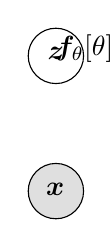
\begin{tikzpicture}[font=\sffamily]
	\node[latent] 							(z) {$\vec z$};
	\node[obs, below=of z] 	(x) {$\vec x$};
	
	\mmedge {z} {x} {$\vec[\theta]{f}$} {left};	
	\mmedge {x} {z} {$\vinv[\theta]{f}$} {right};	
	\end{tikzpicture}
\end{center}
\begin{compactitem}
	\item \textbf{Normalizing}: C.o.V. gives normalized density after applying an invertible transformation.
	\item \textbf{Flow}: Invertible transformations can be composed with each other.
\end{compactitem}
\graybox{
	\vec x
	&\triangleq \vec[M]{z}
	= \vec[\theta]{f}^M \circ \cdots \circ \vec[\theta]{f}^1(\vec[0]{z})
	\triangleq \vec[\theta]{f}(\vec[0]{z}) \\
	\vec[0]{z} 
	&= \lr{ \vec[\theta]{f}^1 }^{-1} \circ \cdots \circ  \lr{ \vec[\theta]{f}^M }^{-1} (\vec x) \\
	p_X(\vec x; \theta)
	&= p_{Z_0}(\vinv[\theta]{f}(\vec x)) \prod_{m=1}^M \bigg|   \det \matr[ (f_{\theta}^m)^{-1} \rightarrow z_m ]{J}  \bigg|
}

\bluesec{Planar Flows}. Invertible transformation
\begin{align}
\vec x 
&= \vecfn[\theta]{f}{z}
= \vec z + \vec u  h\lr{ \innerprod{w}{z} + b  } \\
\left| \det \matr[\vecfn{f}{z} \mapsto \vec z]{J}  \right|
&= \left| \det \lr{ \matr I + h'\lr{ \vec{w}^T \vec z + b }  \vec u \vec{w}^T } \right| \\
&= \left|  1 + h'\lr{ \vec{w}^T \vec z + b }   \vec{u}^T \vec{w}\right|
\end{align}
Note that we need to restrict parameters and non-linearity to ensure the mapping is invertible\footnote{
	For example, let $h = \tanh$. Need to ensure that $\vinv[\theta]{f}(\vec x)$ exists such that
	\begin{align}
	\vinv[\theta]{f}(\vec x) = \vinv[\theta]{f}(\vec z + \vec u \tanh(\vec{w}^T \vec z + b)) &= \vec z
	\end{align} 
	Recall that any function $f$ is invertible IFF it is a bijection. Equivalently, any function $f$ is invertible IFF it is either strictly increasing or decreasing (with no local maxima/minima). Let $\vec z = \vec[\perp]{z} + \vec[\parallel]{z}$, defined relative to $\vec w$, i.e. such that $\vec[\perp]{z}^T \vec w = 0$ and $\vec[\parallel]{z} = \alpha \frac{\vec w}{|| \vec w||^2}$ for some $\alpha \in \R$. This gives
	\begin{align}
	f(\vec z)
	&= \vec[\perp]{z} + \vec[\parallel]{z} + \vec u \tanh \lr{ \vec{w}^T\vec[\parallel]{z} + b  } \\
	\vec{w}^T f(\vec z)
	&= \alpha + \vec{w}^T \vec u \tanh \lr{ \alpha + b  } \triangleq f_{\alpha}(\alpha)
	\end{align}
	Again, note that $f_{\alpha}(\alpha)$ is invertible IFF it's monotonic:
	\begin{align}
	\deriv{f_{\alpha}(\alpha)}{\alpha}
	&= 1 + \vec{w}^T \vec u \tanh ' (\alpha + b) \\
	1 + \vec{w}^T \vec u \tanh ' (\alpha + b) \ge 0 
	&\iff \vec{w}^T \vec u \ge - \inv{\tanh ' (\alpha + b)} 
	\end{align}
	Since $0 < \tanh' (\cdot) \le 1$, we simply need $\vec{w}^T \vec u \ge -1$. The planar flow authors accomplish this via
	\begin{align}
	\hat{u}(w, u)
	&= u + \left[ m(w^T u ) - (w^T u) \right] \frac{w}{||w||^2} \\
	m(x)
	&= -1 + \log \lr{1 + e^x}
	\end{align}
}.

\bluesec{Learning and Inference} \tstamp{1:20:10}. Learning via maximum likelihood over $\mathcal D$:
\graybox{
	\max_{\theta} \log p_X(\mathcal D; \theta)
	&= \sum_{\vec x \in \mathcal D} \log p_Z(\vinv[\theta]{f}(\vec x)) + \log \bigg|  \det \matr[ \vinv{f}(\vec x) \rightarrow \vec x ]{J}  \bigg|
}
\begin{compactitem}[\green{\cmark}]
	\item \textbf{Exact likelihood evaluation} via inverse transformation $\vec x \mapsto \vec z$ and c.o.v. formula (instead of intractable summation over all $\vec z$). 
	\begin{compactitem}[\red{\xmark}]
		\item Requires evaluation of $\det \matr J$, where $J$ is an $n \times n$ Jacobian\footnote{Determinant review: For $3 \times 3$ matrices, you do that technique from physics for calculating vector cross products. For arbitrary $n \times n$ matrices, 
			\begin{align}
			\det A 
			&\triangleq \sum_{c=1}^{N_c} (-1)^{c - 1} a_{11} \det A_{11}
			\end{align}
			where $a_{ij}$ is element at row $i$, column $j$, and $A_{ij}$ is the $(n-1) \times (n-1)$ sub-matrix resulting from removing row $i$ column $j$ from the original matrix $A$. 
		}. Computing such a determinant in general is $\mathcal O(n^3)$. \\
		
		\textbf{Key Idea}: choose transformations s.t. $\matr J$ has special structure allowing for fast computation of $\det J$. For example, if $\matr J$ is triangular, then $\det \matr J = \prod_i J_{ii}$. Conceptually, if $\matr J$ is lower triangular, for example, then $(\forall i, j {>} i)$, $\pderiv{\vinv{f}(\vec x)_i}{x_j} = \pderiv{f(z)_j}{z_i} = 0$. This would be true if e.g. $x_i$ depended only on $z_{\ge i}$. 
	\end{compactitem}
	
	\item \textbf{Sampling} via forward transformation $\vec z \mapsto \vec x$:\marginnote{$\theta = \{ \vec w, \vec u, b \}$}[2em]
	\begin{align}
	\vec z \sim p_Z(\vec z) \qquad \vec x = \vec[\theta]{f}(\vec z)
	\end{align}
	
	\item \textbf{Latent representations} inferred via inverse transformation $\vec z = \vinv[\theta]{f}(\vec x)$. 
\end{compactitem}


\Needspace{25\baselineskip}
\bluesec{Designing Invertible Transformations}. In what follows, we look at two models, NICE and Real-NVP, that have invertible transformations with diagonal Jacobians. \\

\green{NICE}\footnote{Nonlinear Independent Components Estimation (Dinh et al., 2014).} \tstamp{9:00} composes two kinds of invertible transformations:
\begin{compactitem}
	\item \textbf{Additive coupling layers}\footnote{In practice, we assign $d$ randomly for each layer.}. Partition $\vec z$ into two disjoint subsets $\vec[1:d]{z}$ and $\vec[d+1:n]{z}$. for any $1 \le d < n$.
	\begin{align}
	\mgreen{[\vec z \mapsto \vec x ]}	
	\qquad 
	\vec[1:d]{x} &= \vec[1:d]{z} \\
	\vec[d+1:n]{x} &= \vec[d+1:n]{z} + m_{\theta}(\vec[1:d]{z} ) \\
	\mgreen{[\vec x \mapsto \vec z ]}
	\qquad
	\vec[1:d]{z} &= \vec[1:d]{x} \\
	\vec[d+1:n]{z} &= \vec[d+1:n]{x} - m_{\theta}(\vec[1:d]{x} )
	\end{align}
	where $m_{\theta}$ is a NN mapping $d$ inputs to $n - d$ outputs. Jacobian of forward mapping:
	\begin{align}
	\matr[\vec x \rightarrow \vec z]{J}
	&\triangleq \pderiv{\vec x}{\vec z}
	= \begin{pmatrix}
	\matr[d]{I} & \matr 0 \\
	\pderiv{\vec[d+1:n]{x}}{\vec[1:d]{z}  } & \matr[n-d]{I} \\
	\end{pmatrix}
	\\
	\det J &= 1
	\end{align}
	\green{Volume preserving transformation} since det is 1 \tstamp{17:17}. 
	
	\item \textbf{Rescaling layers} (final layer). The forward/inverse mappings and $J$:
	\begin{align}
	\mgreen{[\vec z \mapsto \vec x ]}
	\qquad 
	x_i &= s_i z_i \\
	\mgreen{[\vec x \mapsto \vec z]}
	\qquad 
	z_i &= \frac{x_i}{s_i} \\
	\matr[\vec x \mapsto \vec z]{J}
	&= \text{diag}(\vec s)
	\end{align}
	where $s_i > 0$ is the scaling factor of the $i$th dimension. 
	
\end{compactitem}

\Needspace{10\baselineskip}
\green{Real-NVP}\footnote{Non-volume preserving extension of NICE.}. Coupling layers now shift \textit{and} scale.
\begin{align}
\mgreen{[\vec z \mapsto \vec x ]}	
\qquad 
\vec[1:d]{x} &= \vec[1:d]{z} \\
\vec[d+1:n]{x} &= \vec[d+1:n]{z} \odot \exp\lr{ \alpha_{\theta} \lr{ \vec[1:d]{z}  }  } + \mu_{\theta}(\vec[1:d]{z}) \\
\mgreen{[\vec x \mapsto \vec z ]}
\qquad
\vec[1:d]{z} &= \vec[1:d]{x} \\
\vec[d+1:n]{z} &= \lr{ \vec[d+1:n]{x} - \mu_{\theta}(\vec[1:d]{x} ) } \odot \lr{
	\exp\lr{
		-\alpha_{\theta}\lr{ \vec[1:d]{x} }
	}
}\\
\matr[\vec x \rightarrow \vec z]{J}
&\triangleq \pderiv{\vec x}{\vec z}
= \begin{pmatrix}
\matr[d]{I} & \matr 0 \\
\pderiv{\vec[d+1:n]{x}}{\vec[1:d]{z}  } & \mred{ \text{diag} \lr{ \exp \lr{ \alpha_{\theta} \lr{ \vec[1:d]{z} }  } }  } \\
\end{pmatrix}
\\
\det J
&= \prod_{i=d+1}^{n} \exp \lr{ \alpha_{\theta} \lr{ \vec[1:d]{z} }_i } \\
&=  \exp \lr{ \sum_{i=d+1}^{n} \alpha_{\theta} \lr{ \vec[1:d]{z} }_i } 
\end{align}

\Needspace{25\baselineskip}
\bluesec{Autoregressive Models as Flow Models} \tstamp{43:00}. Consider a Gaussian AR model:
\begin{align}
p(\vec x)
&= \prod_{i=1}^n p(x_i \mid \vec[<i]{x}) \\
&=  \prod_{i=1}^n \Gauss{x_i ;  \mu_i, \exp(\alpha_i)^2 }
\end{align}
where both $\mu_i$ and $\alpha_i$ are functions (neural nets) of $x_1, \ldots x_{i-1}$ (constants for $i \eq 1$). The sampling procedure is defined as follows:
\begin{compactenum}
	\item Sample $z_i \sim \Gauss{0, 1}$ for $i = 1, \ldots, n$. 
	\item Set $x_1 := \exp(\alpha_1) z_1 + \mu_1$. 
	\item For $i$ in $[2..n]$ (inclusive): do
	\begin{compactenum}
		\item Compute $\mu_i(x_1, \ldots, x_{i-1})$ and $\alpha_i(x_1, \ldots, x_{i-1})$.
		\item Set $x_i := \exp(\alpha_i) z_i + \mu_i$. 
	\end{compactenum}
\end{compactenum}
\begin{definition}{Flow Interpretation \tstamp{45:57}}
	Sampled each $z_i$ from a (simple) Gaussian, $\Gauss{0, 1}$. Sampled the associated $x_i$ via invertible transformations parameterized by $\mu_i(\cdot), \alpha_i(\cdot)$.
\end{definition}

We've just described the \green{Masked Autoregressive Flow} (MAF) \tstamp{46:11} model. The sampling for the forward mapping $\vec z \mapsto \vec x$ is illustrated below.

\myfig[0.4\textwidth]{figs/maf.png}

\bluesec{Inverse Autoregressive Flow} (IAF) \tstamp{52:00}. 


\begin{definition}{Probability Density Distillation}
	Student distribution is trained to minimize $D_{KL}$ between student $s$ and teacher $t$:
	\begin{align}
	\dkl{s}{t}
	&= \E[\vec x \sim s]{\log s(\vec x) - \log t(\vec x)}
	\end{align}
\end{definition}

\begin{algorithm}[Parallel Wavenet]
	\textbf{Training}.
	\begin{compactenum}
		\item Train teacher model (\green{MAF}) via MLE.
		\item Train student model (\green{IAF}) to minimize $D_{KL}$.
	\end{compactenum}
	
	\textbf{Testing}. Use student model. \\
	
	Improves sampling efficiency over Wavenet by 1000x!
\end{algorithm}






\begin{example}[Change of Variables: Derivation]
	\textit{Given some [continuous] $\vec z \sim p_Z$, and monotonic $\vecfn{f}{z} = \vec x$, derive $p_X(\vec x)$. Both $\vec z$ and $\vec x$ must have the same dimension.}
	\tcblower
	
	\begin{enumerate}
		\item The density for continuous RV $\vec z$ is defined as
		\begin{align}
		p_Z(\vec z) \triangleq \pderiv{P(Z \le \vec z)}{\vec z}
		\end{align}
		
		\item Since $\vecfn{f}{z}$ is monotonic, we know that\footnote{This part is intuitively clear to me, yet I'm not sure how I'd actually \textit{prove} it.} the CDF for $X$ can be defined in terms of the CDF for $Z$ as
		\begin{align}
		P(X \le \vec x)
		&= P\lr{  Z \in \{  \vec z | \vecfn{f}{z} \le x  \}  }
		\end{align}
		
		\item We can use the above, along with the fact that any monotonic function is invertible, to define the density $p_X(\vec x)$ as
		\begin{align}
		p_X(\vec x)
		&\triangleq \pderiv{P(X \le \vec x) }{\vec x} \\
		&= \pderiv{ P\lr{  Z \in \{  \vec z | \vecfn{f}{z} \le \vec x \}  } }{\vec x} \\
		&= \pderiv{ P\lr{  Z \in \{  \vec z | \vecfn{f}{z} \le \vec x  \}  } }{\vec z} \pderiv{\vec z}{\vec x} \\
		&= \pderiv{ P\lr{  Z  \le \vinv{f}(\vec x)  } }{\vec z} \pderiv{\vec z}{\vec x} \\
		&= p_Z(\vinv{f}(\vec x)) \pderiv{\vec z}{\vec x} \\
		&=p_Z(\vinv{f}(\vec x)) \matr[\vec z \rightarrow \vec x]{J}
		\end{align}
	\end{enumerate}
	
	In summary, the density $p_X(\vec x)$, where $\vec x = \vecfn{f}{z}$, can be written as:
	\graybox{
		p_X(\vec x)
		&= p_Z\lr{\vec z \eq \vinv{f}(\vec x)}
	}
	
	\red{TODO: FINISH THIS AFTER THE STATS BOOKS ARRIVES}
\end{example}


\clearpage
% ----------------------------------------
\subsub{Homework 3}
% ----------------------------------------

\bluesec{Problem 1: Flow Models}. Implement a \green{Masked Autoregressive Flow} (MAF) model. MAF models are themselves composed of \green{Masked Autoregressive Distribution Estimator} (MADE) blocks (each $\vecfn{f}{\cdot}$ will be a MADE block).

\begin{small}
	\lstset{language=Python}
	\begin{lstlisting}
	nf_blocks = []
	for i in range(self.n_flows):
		nf_blocks.append(
			MADE(self.input_size, self.hidden_size, self.n_hidden))
		nf_blocks.append(PermuteLayer(self.input_size))  # permute dims
	self.nf = nn.Sequential(*nf_blocks)
	\end{lstlisting}
\end{small}
Each MADE block is consists of some number of hidden layers, each with an associated mask. 
\begin{compactitem}
	\item \textbf{Forward Pass $[\vec z \mapsto \vec x]$}: Assuming that $\vec z$ comes from some base noise distribution like $\Gauss{0, I}$ (\red{is this still valid when e.g. $\vec z$ is just the output of the previous layer (as in MAF)}), we can use the reparameterization trick for Gaussian sampling to obtain each $x_i$:
	\begin{align}
		x_1 &= \mu_1 + z_1 \exp\lr{ \alpha_1 } \\
		x_2 &= \mu_2(x_1) + z_2 \exp\lr{ \alpha_2(x_1) } \\
		&\vdots \\
		x_n &= \mu_2(x_1, \ldots, x_{n-1}) + z_n \exp\lr{ \alpha_n(x_1, \ldots, x_{n-1}) }
	\end{align}
	Since this is an invertible transformation,
	\begin{align}
		\log \bigg|  \det \pderiv{ \vec z }{  \vec x }  \bigg|
			&= \log \bigg|  \det \pderiv{ \vec x }{  \vec z }  \bigg|^{-1} \\
			&= \log \bigg|  \prod_{i=1}^{n} \exp \lr{\alpha_i }  \bigg|^{-1} \\
			&= - \insum \alpha_i
	\end{align}
	Note that everything we've seen so far has been within a single MADE layer. Our full MAF model consists of 5 such MADE layers.
\end{compactitem}

% ------------------------------------------------------------------------------
\lecture{Lectures}{Generative Adversarial Networks}{October 21, 2019}

\vspace{-1em}
\bluesec{Recap} \tstamp{8:00}. We've seen the following model families so far:
\begin{compactitem}
	\item \green{Autoregressive Models}: $p_{\theta}(x) = \prod_i^n p_{\theta}(x_i \mid x_{<i})$. \textbf{Pro}: tractable likelihoods. \textbf{Con}: no direct mechanism for learning features. 
	
	\item \green{VAEs}: $p_{\theta}(x) = \int p_{\theta}(x, z) \mathrm{d} z$. \textbf{Pro}: can learn feature representations (via latent $z$). \textbf{Con}: intractable marginal likelihoods.
	
	\item \green{Normalizing Flow Models}: $p_{\theta, X}(\vec x) = p_{\theta, Z}(\vinv[\theta]{f}(\vec x)) \big| \det \matr[\vec z \rightarrow \vec x]{J} \big|$
\end{compactitem}
All the above are based on maximizing likelihoods (or approximations).

\begin{example}[Example: great $\log \textprob{test}{\vec x}$; poor samples \tstamp{12:14}]
	Consider a noise mixture model $p_{\theta}(\vec x)$ where $\vec x$ is some $d_x$-dimensional vector, with sampling procedure
	\begin{compactenum}
		\item Sample binary-valued $b \sim \text{Bern}(0.01)$. 
		\item If $b = 1$ (probability 1 percent), then return sample $\vec x \sim p_{data}(\vec x)$. 
		\item Else, return sample $\vec x \sim p_{noise}(\vec x)$.
	\end{compactenum}

	Note that the above procedure can be written as 
	\begin{align}
		p_{\theta}(\vec x) 
			&= 0.01 \textprob{data}{\vec x} + 0.99 \textprob{noise}{\vec x} 
	\end{align}
	
	In what follows, we find an upper and lower bound on $\log p_{\theta}(\vec x)$ to prove it can have great likelihoods.
	
	\begin{align}
		\mgreen{ \log \ptheta{\vec x} }
			&= \log \lr{
				0.01 \textprob{data}{\vec x} + 0.99 \textprob{noise}{\vec x} } \\
			&\ge \log 0.01 \textprob{data}{\vec x} \\
			&= \log \textprob{data}{\vec x} - \log 100
		\\
		\E[p_{data}]{ \mgreen{ \log \ptheta{\vec x} } }
			&\ge \E[p_{data}]{\log \textprob{data}{\vec x}} - \log 100 \\
		\E[p_{data}]{\log \textprob{data}{\vec x}}
			&\ge \E[p_{data}]{\mgreen{\log \ptheta{\vec x}}}
	\end{align}
	where the last line is true because $\dkl{p_{data}}{p_{\theta}} \ge 0$. This gives us the following upper and lower bound:
	\begin{align}
		\E[p_{data}]{\log \textprob{data}{\vec x}}
		\ge \E[p_{data}]{\mgreen{\log \ptheta{\vec x}}}
		\ge \E[p_{data}]{\log \textprob{data}{\vec x}} - \log 100
	\end{align}
	For larger and larger $d_x$, the absolute values of $\log \textprob{data}{\vec x}$ increases\footnote{Think about it. Higher dimensional spaces have more unique possible values for $\vec x$. For higher dimensional spaces, the observed points $\vec x$ represent a much smaller fraction of the total number of points, and will thus likely get assigned lower probabilities (and thus larger $| \log p |$) than e.g. observed data in small dimensional spaces.}. and the contribution of $-\log100$ becomes less and less significant, until 
	\begin{align}
	 \E[p_{data}]{\mgreen{\log \ptheta{\vec x}}}
	 	&\approx 	\E[p_{data}]{\log \textprob{data}{\vec x}}
	\end{align}
	which results in a model with great likelihoods, but horrible samples (mostly noise).
\end{example}


\bluesec{Towards likelihood-free learning} \tstamp{11:23}. GANs can be motivated by asking whether optimizing \textit{likelihoods} is a good approach. There exist cases where model can generate poor samples with great likelihoods, and vice-versa. For example, memorizing training set can result in great samples, but have horrible test likelihoods. Can we disentangle likelihoods and samples?

\begin{itemdefinition}{Two-Sample Tests \tstamp{23:48}}
	\item Given $S_1 = \{\vec x \sim P\}$ and $S_2 = \{\vec x \sim Q\}$, a \green{two-sample test} considers the following hypotheses:
	\begin{compactitem}
		\item Null hypothesis $H_0 : P = Q$. 
		\item Alternate hypothesis $H_1: P \ne Q$. 
	\end{compactitem}

	\item Test statistic $T$ compares $S_1$ and $S_2$ (e.g. difference in means)\footnote{We interpret large $T$ as meaning the samples appear to come from \textit{different} distributions, and low $T$ as meaning the samples appear to come from the \textit{same} distribution}. 
	
	\item If $T < \alpha$, then accept $H_0$ else reject it.
	
	\item \textbf{Key observation}: $T$ is \textit{likelihood-free} since it doesn't involve densities $P$ or $Q$ (only samples). 
\end{itemdefinition}


\bluesec{GANs} \tstamp{30:40}. Key idea: \textit{learn} a statistic that \textit{maximizes} a suitable notion of distance between $S_1$ and $S_2$\footnote{The wording is subtle/confusing here. What we mean is we want to somehow learn a high-quality statistic $T$ that's very large when the samples are not from the same distribution. Why? Because such a $T$ makes the task of minimizing its value (job of the generator) difficult. If $T$ was low to begin with, there wouldn't be much of a task. Stated another way: given that $G$ wants to \textit{minimize} the test statistic, the job of $D$ is to \textit{find} a test statistic that is hard for $G$ to minimize.}. GANs involve a two player minimax game between a \textbf{generator} $G_{\theta}$ and a \textbf{discriminator}


\begin{drawing}
	\node[latent] 							(z) {$\vec z$};
	\node[obs, below=of z] 	(x) {$\vec x$};
	\medge {z} {x} {\hspace{-3em}$G_{\theta}$};
	
	\node[obs, right= of z] 							(z2) {$\vec y$};
	\node[obs, below=of z2] 	(x2) {$\vec x$};
	\medge {x2} {z2} {\hspace{-3em}$D_{\phi}$};
\end{drawing}

\begin{compactitem}
	\item \textbf{Generator} $G_{\theta}: \vec z \mapsto \vec x$. Deterministic directed LVM. \purple{Minimizes} the two-sample test objective in support of $H_0 : p_{data} = p_{\theta}$.
	
	\item \textbf{Discriminator} $D_{\phi} : \vec x \mapsto \vec y$ where $\vec y$ is a binary RV. \red{Maximizes} the two-sample test objective in support of $H_1 : p_{data} \ne p_{\theta}$. For fixed $G$, the discriminator $D$ is performing binary classification with cross entropy. 
\end{compactitem}

\Needspace{10\baselineskip}
The GAN objective function is defined as \tstamp{38:00}
\graybox{
	\mpurple{\min_{\theta}} \mred{\max_{\phi}} V(\mpurple{G_{\theta}}, \mred{D_{\phi}})
		&= \E[\vec x \sim p_{data}]{\log \mred{D_{\phi}}(\vec x)} 
			+ \E[\vec z \sim p(\vec z)]{\log (1 - \mred{D_{\phi}}( \mpurple{G_{\theta}} (\vec z)))}
}

\begin{definition}{Optimal Discriminator}
	The optimal discriminator function $D$ for a given generator $G$ is
	\begin{align}
		D^*_G(\vec x) &= \dfrac{
			p_{data}(\vec x)
		}{ p_{data}(\vec x) + p_G(\vec x)}
	\end{align}
	If we plug this into $V(G, D)$, we obtain
	\begin{align}
		V(G, D^*_G(\vec x))
			&= 2 \djsd{p_{data}}{p_G} - \log 4 \\
		\djsd{p}{q}
			&\triangleq \onehalf \lr{
				\dkl{p}{ \frac{p+q}{2}} + 	\dkl{q}{ \frac{p+q}{2}}
		}
	\end{align}
	where $\djsd{p}{q}$ is the \green{Jensen-Shannon Divergence}\footnote{Properties of $\djsd{p}{q}$:
		\begin{align}
		\djsd{p}{q}	
		&\ge 0 \\
		\djsd{p}{q}
		&= 0 \quad \text{iff} \quad p = q \\
		\djsd{p}{q}
		&= \djsd{q}{p} \\
		\sqrt{\djsd{p}{q}}
		&\le \sqrt{\djsd{p}{r}} + \sqrt{\djsd{r}{q}}
		\end{align}
	}.
\end{definition}
	

\begin{algorithm}[The GAN Training Algorithm \tstamp{52:00}]
	\begin{compactenum}
		\item Sample minibatch of $m$ training points from data.
		$$
		\ivec[1]{x}, \ivec[2]{x}, \ldots, \ivec[m]{x} \sim \mathcal D
		$$
		
		\item Sample minibatch of $m$ noise vectors from $p_Z$.
		$$
		\ivec[1]{z}, \ivec[2]{z}, \ldots, \ivec[m]{z} \sim p_Z
		$$
		
		\item Update generator parameters $\mpurple \theta$ by stochastic gradient \purple{descent}. 
		\begin{align}
			\nabla_{\theta} V(G_{\theta}, D_{\phi})
				&= \inv{m} \nabla_{\theta} \sum_{i=1}^m \log \lr{ 1 - D_{\phi}\lr{ G_{\theta} \lr{  \ivec[i]{z} }  }  }
		\end{align}
		
		\item Update discriminator parameters $\mred \phi$ by stochastic gradient \red{ascent}. 
		\begin{align}
			\nabla_{\phi} V(G_{\theta}, D_{\phi})	
				&= \inv{m} \nabla_{\phi} \sum_{i=1}^m \left[
					\log D_{\phi}\lr{ \ivec[i]{x} }
					+ \log \lr{  1 - D_{\phi}\lr{ G_{\theta}\lr{  \ivec[i]{z} }  } }
				\right]
		\end{align}
		
		\item Repeat for fixed number of epochs.
	\end{compactenum}
\end{algorithm}

\bluesec{Challenges}. 
\begin{compactitem}
	\item \textbf{Unstable Optimization}. $G$ and $D$ often oscillate during training without converging. No robust stopping criteria.
	
	\item \textbf{Mode Collapse} \tstamp{1:11:00}. Generator collapses to one or few samples (dubbed as ``modes''). For example, if $p_{data}$ is multimodal, the generator may collapse to modeling just one of these modes.
	
	\item \textbf{Evaluation}.
\end{compactitem}

\vspace{-1em}
\bluesec{Beyond KL and JSD}. 
\begin{compactitem}
	\item $\dkl{p}{q}$: used by AR and Flow models.
	
	\item $\djsd{p}{q}$ (scaled \& shifted): original GAN objective.
\end{compactitem}

\begin{definition}{f-divergence \tstamp{8:30}}
	Given two densities $p$ and $q$, the \green{f-divergence} is given by
	\begin{align}
		\df{p}{q}
			&\triangleq \E[\vec x \sim q]{f\lr{
				\frac{p(\vec x)}{q(\vec x)}
		}}
	\end{align}
	where $f$ is any convex, \purple{lower-semicontinuous}\footnote{Ok, I understand this now. Remember how piecewise functions over real numbers are defined like
		\begin{align}
			f(x) &= 
			\begin{cases}
				1 & x < 0 \\
				-1 & x \ge 0
			\end{cases}
		\end{align}
		In particular, we say that $f(0) = -1$, while $f(0+\epsilon) = 1$. For this reason, we say $f$ is \purple{lower-semicontinuous}, because $\forall x$, the ``function value'' at $x$ is either literally just $f(x)$ (true everywhere if e.g. $f$ were continuous), or it's larger. Stated even more sloppily, it just means that whenever you try to evaluate $f$ at $x$, you are guaranteed to get back exactly $f(x)$ or a value that's larger than $f(x)$ (which occurs if you are at a discontinuity).
	} function with $f(1) = 0$. Note that if $f(u) = u \log u$, $\df{p}{q} \equiv \dkl{p}{q}$.
\end{definition}

\begin{definition}{Fenchel Conjugate (Complex Conjugate)}
		For any function\footnote{Technically, any function $f : X \mapsto \R \cup \{ -\infty, +\infty \}$ where $X$ is a real vector space. Similarly $f^*: X^* \mapsto \R \cup \{-\infty, +\infty\}$, where $X^*$ is the dual space to $X$.} $f(\cdot)$, its \green{Fenchel conjugate} (a.k.a. the complex conjugate) is defined as\footnote{Recall that the \green{supremum} of a set $S \subset T$ is the smallest element of $T$ that's greater than or equal to all elements in $S$.}
		\begin{align}
			f^*(t)
				&\triangleq\sup_{u \in \text{dom}_f} \lr{ ut - f(u)  } 
		\end{align}
		\begin{compactitem}
			\item $f^*$ is always lower semi-continuous. 
			\item $f^{**} = f$ IFF $f$ is convex and lower semi-continuous.
		\end{compactitem}
		
\end{definition}

\Needspace{10\baselineskip}
To use $f$-divergences as our 2-sample test objective for likelihood-free learning, we need to be able to estimate it only via samples\footnote{Why can't we already? Technically, all MLE applications minimize $\dkl{p_{data}}{p_{\theta}}$ but (obviously) never have direct access to $p_{data}$. Confused in general by the notion of likelihood-free learning, since it seems no different \textit{in practice} (as opposed to in theory/formulas)}. We can obtain a lower bound that is likelihood-free wrt $p$ and $q$ to any $f$-divergence via its Fenchel conjugate \tstamp{20:00}. 
\begin{align}
	\df{p}{q}
		&\triangleq \E[\vec x \sim q]{
				f\lr{
				\frac{p(\vec x)}{q(\vec x)} 
			}} \\
		&= \E[\vec x \sim q]{
			f^{**}\lr{
				\frac{p(\vec x)}{q(\vec x)} 
		}} \\
		&=  \E[\vec x \sim q]{
			\sup_{t \in \text{dom}_{f^*}} \lr{ t \frac{p(\vec x)}{q(\vec x)}   - f^*(t)  } 
		} \\
		&:= \E[\vec x \sim q]{
			\mgreen{T(\vec x)} \frac{p(\vec x)}{q(\vec x)} - f^*\lr{ \mgreen{T(\vec x)}  }
		} \\
		&= \int \mathrm{d}\vec x \left[
			\mgreen{T(\vec x)} p(\vec x) - f^*\lr{ \mgreen{T(\vec x)} } q(\vec x)
		\right] \\
		&\ge \sup_{\mpurple{\hat T} \in \mathcal T} 
			\int \mathrm{d}\vec x \left[
				\mpurple{\hat{T}(\vec x)} p(\vec x) - f^*\lr{ \mpurple{\hat{T}(\vec x)} } q(\vec x)
			\right] \\
	&= \sup_{\mpurple{\hat T} \in \mathcal T} \lr{
		\E[\vec x \sim p]{  \mpurple{\hat T(\vec x)}  }
		- \E[\vec x \sim q]{f^*\lr{ \mpurple{\hat T\lr{\vec x}  }  } }
	}		
\end{align}
where $\mathcal T : \mathcal X \mapsto \R$ is an arbitrary class of functions. 


\bluesec{f-GAN: Variational Divergence Minimization}. We can rewrite the result above, plugging in $p := p_{data}$, $q := p_{G_{\theta}}$, $\hat T := T_{\phi}$, to obtain 
\graybox{
	\df{p}{q}
		&\ge \sup_{\mpurple{\hat T} \in \mathcal T} \lr{
		\E[\vec x \sim p]{  \mpurple{\hat T(\vec x)}  }
		- \E[\vec x \sim q]{f^*\lr{ \mpurple{\hat T\lr{\vec x}  }  } }
	} \\
	\min_{\theta} \max_{\phi} F(\theta, \phi)
		&= \E[\vec x \sim p_{data}]{T_{\phi}(\vec x)} - \E[\vec x \sim p_{G_{\theta}}]{f^*\lr{  T_{\phi}\lr{\vec x}  } }	
}
where the interpretations of $\phi$ (discriminator) and $\theta$ (generator) are consistent with our original GAN formulation\footnote{For convenience:  
\begin{align}
	\mpurple{\min_{\theta}} \mred{\max_{\phi}} V(\mpurple{G_{\theta}}, \mred{D_{\phi}})
	&= \E[\vec x \sim p_{data}]{\log \mred{D_{\phi}}(\vec x)} 
	+ \E[\vec z \sim p(\vec z)]{\log (1 - \mred{D_{\phi}}( \mpurple{G_{\theta}} (\vec z)))}
\end{align}
}

\bluesec{Inferring Latent Representations in GANs} \tstamp{30:50}. Unlike\textellipsis
\begin{compactitem}
	\item Normalizing flow models: $\vec z = \vinv[\theta]{f}(\vec x)$.
	
	\item VAEs: $\vec z \sim q_{\phi}(\vec z \mid \vec x)$.
\end{compactitem}
\textellipsis the GAN generator is a directed LVM $\vec z \mapsto \vec x$ and it need not be invertible. In practice, there are a few ways to get latent representations \tstamp{32:00}:
\begin{compactitem}
	\item[\gray{\RIGHTarrow}]  [Use $D$] For any point $\vec x$, use the activations of the prefinal layer of $D$ as feature representation\footnote{\red{What? How is this even remotely a valid approach? What does the prefinal layer have to $\vec z$??}}
	
	\item[\gray{\RIGHTarrow}] [Change learning algorithm] Compare samples of $\lr{ \vec z, \vec x}$ (instead of just $\vec x$) from joint distributions of model/data. Note that we don't have access to $\vec z$ for the $\vec x$ sampled from $p_{data}$. 
\end{compactitem}

\bluesec{BiGAN} \tstamp{35:00}. Introduces an encoder $E : \vec x \mapsto \vec z$ to obtain latent representation from $\vec x \sim \textprob{data}{\vec x}$.
\begin{compactitem}
	\item Discriminator maximizes two-sample test objective between $\lr{\vec z, G(\vec z) }$ and $\lr{ E(\vec x), \vec x }$. 
	
	\item After training, we can \textbf{sample} $\vec x \sim p_{G_{\theta}}(\vec x)$ (as usual), but now we can also \textbf{infer} $\vec z = E(\vec x)$.
\end{compactitem}

\myfig[0.5\textwidth]{figs/bigan.png}



\bluesec{CycleGAN}. Adversarial training across two domains. Setting: we have unpaired sets of samples $X \in \mathcal X$ and $Y \in \mathcal Y$. Can we translate $\mathcal X \rightleftarrows \mathcal Y$ in an unsupervised manner? \green{CycleGAN} learns two parameterized conditional generative models:
\begin{align}
	G : \mathcal X \mapsto \mathcal Y 
		\qquad &
	F : \mathcal Y \mapsto \mathcal X \\
	F(G(X)) \approx X \qquad &
	G(F(Y)) \approx Y
\end{align}
Discriminator $D_Y$ compares observed $Y$ with samples $\hat Y = G(X)$, while $D_X$ compares observed $X$ with samples $\hat X = F(Y)$. The CycleGAN loss function is as follows, where for brevity I've defined $\mathcal{L}\lr{ G, D_Y} = \mathcal{L}_{\text{GAN}}\lr{ G, D_Y, X, Y }$
\graybox{
	\min_{F, G, D_X, D_Y} &
		\mathcal{L}_G + 
		\mathcal{L}_F +
		\lambda \lr{  
		\E[X]{ ||F(G(X)) - X ||_1 } + \E[Y]{||  G(F(Y)) - Y ||_1}
	} \\
	\mathcal{L}_G 
		&:= \mathcal{L}_{\text{GAN}}\lr{ G, D_Y, X, Y } \\
	\mathcal{L}_F 
		&:= \mathcal{L}_{\text{GAN}}\lr{ F, D_X, X, Y }
}










% ------------------------------------------------------------------------------
\lecture{Lectures}{Energy-Based Models I}{October 28, 2019}



Say we have some function $g_{\theta}(x)$ and we want to model $p(x)$. This obviously means we must satisfy:
\begin{align}
	g_{\theta}(x) &\ge 0 \quad \forall x \\
 	\int g_{\theta}(x) \mathrm{d} x &= 1
\end{align}
We'll be referring to the integral above as the \textit{volume} of $g_{\theta}$. We typically choose $g_{\theta}$ s.t. we know the volume \textit{analytically}, e.g. 
\begin{align}
	\mtgreen{[Gaussian]}
	\qquad 
	g_{\mu, \sigma}(x) 
		&= e^{- \frac{ (x - \mu)^2 }{ 2\sigma^2  }} \longrightarrow \sqrt{2\pi \sigma^2} \\
	\mtgreen{[Exponential]}
	\qquad 
	g_{\lambda}(x)
		&= e^{-\lambda x} \longrightarrow \inv{\lambda}
\end{align}


\bluesec{Energy-Based Model}. ``Give up'' on computing volume analytically and just do:
\graybox{
	p_{\theta}(x)
		&= \inv{Z(\theta)} \exp \lr{    f_{\theta}\lr{x} } \\
	Z(\theta)
		&= \int \exp \lr{  f_{\theta}\lr{x} } \mathrm{d} x
}
Exponentials allow us to work in log-probability space with $f_{\theta}$. Allows for capturing large variations in probability. Also because exponential families, etc. In physics, $-f_{\theta}(x)$ represents the \green{energy}. 

\begin{compactitem}
	\item[\green{\cmark}] Extremely flexible. Works with basically any $f_{\theta}$.
	\item[\red{\xmark}] Sampling from $p_{\theta}(x)$ is hard.
	\item[\red{\xmark}] Evaluating/optimizing likelihood $p_{\theta}(x)$ is hard (learning is hard).
	\item[\red{\xmark}] No feature learning.
	\item[\red{\xmark}] Computing $Z(\theta)$ scales exponentially in dimensionality of $x$.
\end{compactitem}

\bluesec{Applications}. Note that probability ratios for two points $x$ and $x'$ don't require knowing $Z(\theta)$:
\begin{align}
	\frac{  p_{\theta}(x)  }{ p_{\theta}(x')  }
		&= \exp \lr{  f_{\theta}\lr{x}  -  f_{\theta}\lr{x'} }
\end{align}
Useful for e.g. anomaly detection and denoising.


\bluesec{Training}. Goal: maximize $f_{\theta}(x_{train}) / Z(\theta)$ by increasing numerator, decreasing denominator. \green{Contrastive divergence} uses MC estimates to approximate $Z(\theta)$. Takes gradients $\nabla_{\theta}(f_{\theta}(x_{train})  - f_{\theta}(x_{sample}) )$.






% ==================================================================================
% CONCEPTS
% ==================================================================================
\mysection{Concepts}\label{Concepts}


% ------------------------------------------------------------------------------
\lecture{Concepts}{Evidence Lower Bound (ELBo)}{October 20, 2019}

The \green{evidence} (a.k.a. the marginal likelihood) is defined as $p(x) = \sum_z p(x, z)$. The goal here to find a \textit{lower bound} on the evidence. Computing the evidence is typically intractable, due to the expectation over latent variables:
\begin{align}
	\log p_{\theta}(x)
		&= \log \E[z \sim q(z)]{\frac{ p_{\theta}(x, z)  }{ q(z)  }} 
\end{align}
Note that the above is true for \textit{any} distribution $q(z)$. 

\begin{definition}{Convex functions and Jensen's Inequality}
	A function $f(x)$ is convex over the interval $[x=a, x=b]$ if every chord of the function lies above the function. That is, $\forall x_1, x_2 \in [a, b]$ and $0 \le \lambda \le 1$:
\begin{align}
f\left(  \lambda x_1 + (1 - \lambda) x_2 \right) &\le \lambda f(x_1) + (1 - \lambda) f(x_2) \\
f\left( \E{x} \right) &\le \E{f(x)} \qquad \mtred{[Jensen's Inequality]} 
\end{align}
\end{definition}

Observe that $\log$ is a \textbf{concave function}. In other words, $\log(\E{x}) \ge \E{\log x}$. This means that $\E{\log x}$ is a \textit{lower bound} on $\log \E{x}$. From above, we see that $\log p_{\theta}(x)$ can be rewritten as a log of an expectation. As such, we define the \green{evidence lower bound (ELBo)}, denoted $\mathcal L(x; \theta, \phi)$, as\footnote{Derivation of $\elbo$ expressed with $D_{KL}$:
\begin{align}
	\dkl{q(z)}{p_{\theta}(z \mid x)}
		&\triangleq \E[q]{\log \frac{q(z)}{p_{\theta}(z \mid x)}} \\
		&= - H(q) - \E[q]{\log p_{\theta}(z  \mid x)} \\
		&= - H(q) - \E[q]{\log p_{\theta}(x, z) / p_{\theta}(x)} \\
		&= - H(q) - \E[q]{\log p_{\theta}(x, z)} + \E[q]{\log p_{\theta}(x)} \\
		&= - H(q) - \E[q]{\log p_{\theta}(x, z)} + \log p_{\theta}(x) \\
		&= -\elbo + \log p_{\theta}(x)
\end{align}
}
\graybox{
	\elbo 
		&\triangleq \E[z \sim q(z)]{\log \frac{ p_{\theta}(x, z) }{ q(z)  }  } \\
		&= \E[z \sim q(z)]{\log p_{\theta}(x, z)} + H(q) \\
		&= \log p_{\theta}(x) - \dkl{q(z)}{p_{\theta}(z \mid x)} \\
		&= \E[z \sim q(z)]{\log p_{\theta}(x \mid z)} - \dkl{q(z)}{p(z)} \label{eq:elbo-vae} \\
	\log p_{\theta}(x) 
		&\ge \elbo  
}

% <><><><><><><> I T E M  D E F I N I T I O N <><><><><><><> 
\RenewDocumentEnvironment{itemdefinition}
{O{-1em} m} % <arg spec> 
{ 	% <start code>
	\IfNoValueTF{#2}{}{\textbf{#2}} \vspace*{#1}
	\begin{quote}
		\small
		\begin{compactitem}[\gray{\RIGHTarrow}]
		}{ % <end code>
		\end{compactitem}
	\end{quote}
}


\Needspace{15\baselineskip}
\begin{itemdefinition}{Questions/Answers}
\QA{Why is a lower bound useful at all?}{
	In this case it's useful because $\log p_{\theta}(x) \eq \elbo$ when $\dkl{q(z)}{p_{\theta}(z \mid x)} \eq 0$. The fact that the formula for $\elbo$ is a lower bound on $\log p_{\theta}(x)$ isn't useful by itself; the useful part is that we can drive $\elbo$ closer and closer to  $\log p_{\theta}(x)$ by minimizing the KL-divergence of $q$ with the posterior $p_{\theta}(z \mid x)$.}

\QA{Why is $\log p(x)$ what we want? Why not just $p(x)$?}{
	idk. Probably because logs are better for computational reasons.}

\QA{Look at the form of $\elbo$ given by \ref{eq:elbo-vae}. It implies that our lower bound gets maximized when $\dkl{q(z)}{p(z)} \rightarrow 0$. Doesn't this just encourage our encoder to learn $p(\vec z)$? How is that even useful (since we already know what $p(\vec z)$ is? What if we just use $p(\vec z)$ directly?)}{
	yo good question idk tho}
\end{itemdefinition}



\end{document}